% Copyright 2006 by Till Tantau
%
% This file may be distributed and/or modified
%
% 1. under the LaTeX Project Public License and/or
% 2. under the GNU Free Documentation License.
%
% See the file doc/generic/pgf/licenses/LICENSE for more details.

% \section{Tutorial: A Picture for Karl's Students}
\section{教程:给 Karl 的学生的一张图}

\bohs

% This tutorial is intended for new users of \tikzname. It
% does not give an exhaustive account of all the features of \tikzname,
% just of those that you are likely to use right away. 
该教程是写给 \tikzname\ 的新手的,它并不详细罗列 \tikzname\ 的所有特性,而是只讲那些你可能立马会用到的。

% Karl is a math and chemistry high-school teacher. He used to create
% the graphics in his worksheets and exams using \LaTeX's |{picture}|
% environment. While the results were acceptable, creating the graphics
% often turned out to be a lengthy process. Also, there tended to be
% problems with lines having slightly wrong angles and circles also
% seemed to be hard to get right. Naturally, his students could not care
% less whether the lines had the exact right angles and they find
% Karl's exams too difficult no matter how nicely they were drawn. But
% Karl was never entirely satisfied with the result.
Karl 是一名高中数学和化学老师,他以前用 \LaTeX\ 的 \ltz{\{picture\}} 环境,为习题和考试画图。
尽管结果可以接受,但是绘图通常要花很久,并且还有一些问题,比如线之间有微小的角度错误,圆形好像也很难画对。
当然,他的学生并不关心线之间的角度对不对,因为 Karl 出的试题太难了,画得再好也没用。
但 Karl 对绘图的结果从不满意。

% Karl's son, who was even less satisfied with the results (he did not
% have to take the exams, after all),  told Karl that he might wish
% to try out a new package for creating graphics. A bit confusingly,
% this package seems to have two names: First, Karl had to download and
% install a package called \pgfname. Then it turns out that inside this
% package there is another package called \tikzname, which is supposed to
% stand for ``\tikzname\ ist \emph{kein}  Zeichenprogramm.'' Karl finds this
% all a bit strange and \tikzname\ seems to indicate that the package
% does not do what he needs. However, having used \textsc{gnu}
% software for quite some time and ``\textsc{gnu} not being Unix,''
% there seems to be hope yet. His son assures him that \tikzname's name is
% intended to warn people that \tikzname\ is not a program that you can
% use to draw graphics with your mouse or tablet. Rather, it is more
% like a ``graphics language.''
Karl 的儿子对绘图结果更不满意(毕竟他不要考试),儿子告诉 Karl 他也许愿意试试一个新的宏包来绘图。
令人困惑的是,这个宏包似乎有两个名字:首先 Karl 需要下载和安装一个叫 \pgfname\ 的宏包,接着他发现这个宏包里还有另一个宏包,叫 \tikzname,应该代表“\tikzname\ ist \emph{kein}  Zeichenprogramm”(\tikzname\ 不是一个画图程序)。Karl 觉得有点奇怪,从 \tikzname\ 的名字来看,似乎并不能满足自己的要求。
不过,由于他用过一段时间的 \textsc{gnu} 软件,并且知道“\textsc{gnu}'s Not Unix!”(\textsc{gnu} 不是 Unix)这句典故,因此似乎有点希望。
他儿子告诉他,\tikzname\ 起这个名字,是为了提醒人们,\tikzname\ 不是一个用鼠标和平板画图的程序,相反,它更像是一门“图形语言”。

\eohs

% \subsection{Problem Statement}
\subsection{问题陈述}

\bohs
% Karl wants to put a graphic on the next worksheet for his
% students. He is currently teaching his students about sine and
% cosine. What he would like to have is something that looks like this
% (ideally):
Karl 想在下次学生习题中放一张图,他现在正在教正弦和余弦。他想得到这样的图(理想情况):

\eohs

\noindent
\begin{tikzpicture}
  [scale=3,line cap=round,
   % Styles
   axes/.style=,
   important line/.style={very thick},
   information text/.style={rounded corners,fill=red!10,inner sep=1ex}]

  % Local definitions
  \def\costhirty{0.8660256}

  % Colors
  \colorlet{anglecolor}{green!50!black}
  \colorlet{sincolor}{red}
  \colorlet{tancolor}{orange!80!black}
  \colorlet{coscolor}{blue}

  % The graphic
  \draw[help lines,step=0.5cm] (-1.4,-1.4) grid (1.4,1.4);

  \draw (0,0) circle [radius=1cm];

  \begin{scope}[axes]
    \draw[->] (-1.5,0) -- (1.5,0) node[right] {$x$};
    \draw[->] (0,-1.5) -- (0,1.5) node[above] {$y$};

    \foreach \x/\xtext in {-1, -.5/-\frac{1}{2}, 1}
      \draw[xshift=\x cm] (0pt,1pt) -- (0pt,-1pt) node[below,fill=white] {$\xtext$};

    \foreach \y/\ytext in {-1, -.5/-\frac{1}{2}, .5/\frac{1}{2}, 1}
      \draw[yshift=\y cm] (1pt,0pt) -- (-1pt,0pt) node[left,fill=white] {$\ytext$};
  \end{scope}

  \filldraw[fill=green!20,draw=anglecolor] (0,0) -- (3mm,0pt) arc(0:30:3mm);
  \draw (15:2mm) node[anglecolor] {$\alpha$};

  \draw[important line,sincolor]
    (30:1cm) -- node[left=1pt,fill=white] {$\sin \alpha$} +(0,-.5);

  \draw[important line,coscolor]
    (0,0) -- node[below=2pt,fill=white] {$\cos \alpha$} (\costhirty,0);

  \draw[important line,tancolor] (1,0) --
    node [right=1pt,fill=white]
    {
      $\displaystyle \tan \alpha \color{black}=
      \frac{{\color{sincolor}\sin \alpha}}{\color{coscolor}\cos \alpha}$
    } (intersection of 0,0--30:1cm and 1,0--1,1) coordinate (t);

  \draw (0,0) -- (t);

  \draw[xshift=1.85cm] node [right,text width=6cm,information text]
    {
      % The {\color{anglecolor} angle $\alpha$} is $30^\circ$ in the
      % example ($\pi/6$ in radians). The {\color{sincolor}sine of
      %   $\alpha$}, which is the height of the red line, is
      在本例中,{\color{anglecolor} 角 $\alpha$} 为 $30^\circ$ (等于 $\pi / 6$ 弧度),{\color{sincolor} $\alpha$ 的正弦},也就是红色线段的高度,为
      \[
      {\color{sincolor} \sin \alpha} = 1/2.
      \]
      % By the Theorem of Pythagoras we have ${\color{coscolor}\cos^2 \alpha} +
      % {\color{sincolor}\sin^2\alpha} =1$. Thus the length of the blue
      % line, which is the {\color{coscolor}cosine of $\alpha$}, must be
      根据勾股定理,我们有 ${\color{coscolor}\cos^2 \alpha} + {\color{sincolor}\sin^2\alpha} =1$。因此蓝色线段的长度,也就是~{\color{coscolor} $\alpha$ 的余弦},肯定为
      \[
      {\color{coscolor}\cos\alpha} = \sqrt{1 - 1/4} = \textstyle
      \sqrt{3}/2.
      \]%
      % This shows that {\color{tancolor}$\tan \alpha$}, which is the
      % height of the orange line, is
      由此可以得到~{\color{tancolor} $\tan \alpha$},也就是橙色线段的高度,为
      \[
      {\color{tancolor}\tan\alpha} = \frac{{\color{sincolor} \sin \alpha}}{{\color{coscolor}\cos \alpha}} = 1/\sqrt 3.
      \]%
    };
\end{tikzpicture}


% \subsection{Setting up the Environment}
\subsection{设置环境}

\bohs

% In \tikzname, to draw a picture, at the start of the picture
% you need to tell \TeX\ or \LaTeX\ that you want to start a picture. In
% \LaTeX\ this is done using the environment |{tikzpicture}|, in plain
% \TeX\ you just use |\tikzpicture| to start the picture and
% |\endtikzpicture| to end it.
要在 \tikzname\ 中画一张图片,你需要在图片开头告诉 \TeX\ 或者 \LaTeX\ 你想开始画一张图。
在 \LaTeX\ 中需要用 \ltz{\{tikzpicture\}} 环境,在 plain \TeX\ 中你只要用 \ltz{\\tikzpicture} 开始图片,再用 \ltz{\\endtikzpicture} 结束图片。

\eohs

% \subsubsection{Setting up the Environment in \LaTeX}
\subsubsection{设置 \LaTeX\ 中的环境}

% Karl, being a \LaTeX\ user, thus sets up his file as follows:
Karl 是一个 \LaTeX\ 用户,所以他的设置是这样的:

\begin{codeexample}[code only]
\documentclass{article} % say
\usepackage{tikz}
\begin{document}
We are working on
\begin{tikzpicture}
  \draw (-1.5,0) -- (1.5,0);
  \draw (0,-1.5) -- (0,1.5);
\end{tikzpicture}.
\end{document}
\end{codeexample}

\bohs

% When executed, that is, run via |pdflatex| or via |latex| followed by
% |dvips|, the resulting will contain something that looks like this:
当程序执行时,也就是用 |pdflatex|,或者是 |latex| 加上 |dvips|,输出包含这样的内容:

\eohs

\begin{codeexample}[width=7cm]
We are working on
\begin{tikzpicture}
  \draw (-1.5,0) -- (1.5,0);
  \draw (0,-1.5) -- (0,1.5);
\end{tikzpicture}.
\end{codeexample}

\bohs

% Admittedly, not quite the whole picture, yet, but we
% do have the axes established. Well, not quite, but we have the lines
% that make up the axes drawn. Karl suddenly has a sinking feeling
% that the picture is still some way off.
诚然,图还算不上完整,不过我们已经建好坐标轴,还画好组成坐标轴的线了。
Karl 突然有点沮丧,似乎离画完还有不少距离。

% Let's have a more detailed look at the code. First, the package
% |tikz| is loaded. This package is a so-called ``frontend'' to the
% basic \pgfname\ system. The basic layer, which is also described in this
% manual, is somewhat more, well, basic and thus harder to use. The
% frontend makes things easier by providing a simpler syntax.
让我们更仔细地看一下代码。首先导入 \ltz{tikz} 库,也就是基础 \pgfname\ 系统所谓的“前端”。
本手册还会提到基本层,更基础也更难用。
这个前端语法更简单,让画图变得更容易了。

% Inside the environment there are two |\draw| commands. They mean:
% ``The path, which is specified following the command up to the
% semicolon, should be drawn.'' The first path is specified
% as |(-1.5,0) -- (0,1.5)|, which means ``a straight line from the point
% at position $(-1.5,0)$ to the point at position $(0,1.5)$.'' Here, the
% positions are specified within a special coordinate system in which,
% initially, one unit is 1cm.
里面有两句 \ltz{\\draw} 命令,意思是:“从此处到逗号间指定的路径,需要画出来。”
第一条路径指定为 \ltz{(-1.5,0) -- (0,1.5)},意思是:“一条从点 $(-1.5,0)$ 到点 $(-1.5,0)$ 的线”。
在这里,位置是用一个特殊的坐标系统指定的,初始的单位长度是 1cm。

% Karl is quite pleased to note that the environment automatically
% reserves enough space to encompass the picture.
Karl 很高兴地注意到,环境中已经预留了足够的空间来容纳图片。

\eohs

% \subsubsection{Setting up the Environment in Plain \TeX}
\subsubsection{设置 Plain \TeX\ 中的环境}

\bohs

% Karl's wife Gerda, who also happens to be a math teacher, is not a
% \LaTeX\ user, but uses plain \TeX\ since she prefers to do things
% ``the old way.'' She can also use \tikzname. Instead of
% |\usepackage{tikz}| she has to write |\input tikz.tex| and instead of
% |\begin{tikzpicture}| she writes |\tikzpicture| and  instead of
% |\end{tikzpicture}| she writes |\endtikzpicture|.
Karl 的妻子 Gerda,恰好也是一名数学老师,她不是 \LaTeX\ 用户,而是用 plain \TeX\ ,因为她更喜欢“老派的方法”。
她也能用 \tikzname,不过不是 \ltz{\\usepackage\{tikz\}},而是 \ltz{\\input tikz.tex},同样,\ltz{\\begin\{tikzpicture\}} 和 \ltz{\\end\{tikzpicture\}} 也应该换成 \ltz{\\tikzpicture} 和 \ltz{\\endtikzpicture}。

% Thus, she would use:
因此她应该用下面的语句:

\eohs

\begin{codeexample}[code only]
%% Plain TeX file
\input tikz.tex
\baselineskip=12pt
\hsize=6.3truein
\vsize=8.7truein
We are working on
\tikzpicture
  \draw (-1.5,0) -- (1.5,0);
  \draw (0,-1.5) -- (0,1.5);
\endtikzpicture.
\bye
\end{codeexample}

\bohs

% Gerda can typeset this file using either |pdftex| or |tex| together
% with |dvips|. \tikzname\ will automatically discern which driver she is
% using. If she wishes to use |dvipdfm| together with |tex|, she
% either needs to modify the file |pgf.cfg| or can write
% |\def\pgfsysdriver{pgfsys-dvipdfm.def}| somewhere \emph{before} she
% inputs |tikz.tex| or |pgf.tex|.
Gerda 既能用 |pdftex| 也能用 |tex| 加 |dvips| 来排版这个文件。
\tikzname\ 会自动识别她用了哪个驱动。
如果她想用 |dvipdfm| 结合 |tex|,她既可以选择修改 |pfg.cfg| 文件,也可以选择在导入 |tikz.tex| 或是 |pgf.tex| 之前加上 \ltz{\\def\\pgfsysdriver\{pgfsys-dvipdfm.def\}}。

\eohs

% \subsubsection{Setting up the Environment in Con\TeX t}
\subsubsection{设置 Con\TeX t 中的环境}

\bohs

% Karl's uncle Hans uses Con\TeX t. Like Gerda, Hans can also use
% \tikzname. Instead of |\usepackage{tikz}| he says
% |\usemodule[tikz]|. Instead of |\begin{tikzpicture}| he writes
%   |\starttikzpicture| and  instead of |\end{tikzpicture}| he writes
% |\stoptikzpicture|.
Karl 的叔叔 Hans 用 Con\TeX t,Hans 也能像 Gerda 一样使用 \tikzname。
他需要把 \ltz{\\usepackage\{tikz\}} 换成 \ltz{\\usemodule[tikz]},同样,\ltz{\\begin\{tikzpicture\}} 和 \ltz{\\end\{tikzpicture\}} 也要换成 \ltz{\\starttikzpicture} 和 \ltz{\\stoptikzpicture}。

% His version of the example looks like this:
他的样例代码像这样:

\eohs

\begin{codeexample}[code only]
%% ConTeXt file
\usemodule[tikz]

\starttext
  We are working on
  \starttikzpicture
    \draw (-1.5,0) -- (1.5,0);
    \draw (0,-1.5) -- (0,1.5);
  \stoptikzpicture.
\stoptext
\end{codeexample}

\bohs

% Hans will now typeset this file in the usual way using
% |texexec| or |context|.
Hans 现在就能像平常一样,用 |texexec| 或者 |context| 来排版这个文件了。

\eohs

% \subsection{Straight Path Construction}
\subsection{直线路径创建}

\bohs

% The basic building block of all pictures in \tikzname\ is the path.
% A \emph{path} is a series of straight lines and curves that are
% connected (that is not the whole picture, but let us ignore the
% complications for the moment). You start a path by specifying the
% coordinates of the start position as a point in round brackets, as in
% |(0,0)|. This is followed by a series of ``path extension
% operations.'' The simplest is |--|, which we used already. It must be
% followed by another coordinate and it extends the path in a straight
% line to this new position. For example, if we were to turn the two
% paths of the axes into one path, the following would result:
\tikzname\ 里所有图片的基本单元是路径(path)。
\emph{路径}就是相连的直线和曲线(并不是整个图片都是如此,不过让我们暂时忽略复杂的部分)。
你指定一个起点作为路径开始,圆括号中为点的坐标,比如 \ltz{(0,0)}。
紧接着是一系列的“路径扩展操作”,最简单的是 \ltz{--},我们之前用过,它后面必须跟着另一个坐标,它将原来的路径沿直线延伸到新的位置。
比如,如果我们打算把坐标轴的两条路径并成一条,那么会得到下面的结果:

\eohs

\begin{codeexample}[]
\tikz \draw (-1.5,0) -- (1.5,0) -- (0,-1.5) -- (0,1.5);
\end{codeexample}

\bohs

% Karl is a bit confused by the fact that there is no |{tikzpicture}|
% environment, here. Instead, the little command |\tikz| is used. This
% command either takes one argument (starting with an opening brace as in
% |\tikz{\draw (0,0) -- (1.5,0)}|, which yields \tikz{\draw (0,0)
%  --(1.5,0);}) or collects everything up to the next semicolon and
% puts it inside a |{tikzpicture}| environment. As a rule of thumb, all
% \tikzname\ graphic drawing commands must occur as an argument of |\tikz|
% or inside a |{tikzpicture}| environment. Fortunately, the command
% |\draw| will only be defined inside this environment, so there is
% little chance that you will accidentally do something wrong here.
Karl 有点困惑,因为这里没见到 \ltz{\{tikzpicture\}} 环境,而是用了一个小命令 \ltz{\\tikz}。
这个命令既可以接受单个参数(放在花括号中,比如 \ltz{\\tikz{\\draw (0,0) -- (1.5,0)}} 会生成一条线 \tikz{\draw (0,0) --(1.5,0);}),
也可以将其放到 |{tikzpicture}| 环境中,每句用以分号结尾。
一般来说,所有的 \tikzname\ 绘图命令必须作为 \ltz{\\tikz} 的参数,或者放在 \ltz{\{tikzpicture\}} 环境里。
幸运的是,\ltz{\\draw} 命令只定义在这种环境下,因此你很少会有出错的机会。

\eohs

% \subsection{Curved Path Construction}
\subsection{曲线路径创建}

\bohs

% The next thing Karl wants to do is to draw the circle. For this,
% straight lines obviously will not do. Instead, we need some way to
% draw curves. For this, \tikzname\ provides a special syntax. One or two
% ``control points'' are needed. The math behind them is not quite
% trivial, but here is the basic idea: Suppose you are at point $x$ and
% the first control point is $y$. Then the curve will start ``going in
% the direction of~$y$ at~$x$,'' that is, the tangent of the curve at $x$
% will point toward~$y$. Next, suppose the curve should end at $z$ and
% the second support point is $w$. Then the curve will, indeed, end at
% $z$ and the tangent of the curve at point $z$ will go through $w$.
Karl 下一步想做的就是画圆,很明显用直线做不到,所以我们需要一些方法绘制曲线。
为此,\tikzname\ 提供了一个特殊的语法,需要用一到两个“控制点”。
它背后的数学并不简单,但是基本思想是:
假设你位于点 $x$,第一个控制点是 $y$,那么曲线开始时会沿着从 $x$ 到 $y$ 的方向,也就是说,该曲线在点 $x$ 处的切线经过 $y$。
接着,假设曲线的结束点为 $z$,第二个控制点是 $w$,那么该曲线就会在点 $z$ 处结束,并且曲线在点 $z$ 处的切线经过 $w$。

% Here is an example (the control points have been added for clarity):
例子如下(为了更清楚地说明,这里画上了控制点):

\eohs

\begin{codeexample}[]
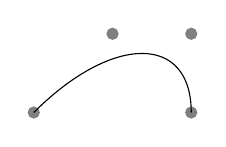
\begin{tikzpicture}
  \filldraw [gray] (0,0) circle [radius=2pt]
                   (1,1) circle [radius=2pt]
                   (2,1) circle [radius=2pt]
                   (2,0) circle [radius=2pt];
  \draw (0,0) .. controls (1,1) and (2,1) .. (2,0);
\end{tikzpicture}
\end{codeexample}

\bohs

% The general syntax for extending a path in a ``curved'' way is
% |.. controls| \meta{first control point} |and| \meta{second control
%   point} |..| \meta{end point}. You can leave out the |and|
% \meta{second control point}, which causes the first one to be used
% twice.
以曲线方式延伸路径的通用语法是~{\color{blue} \ltz{.. controls}  \metazh{第一个控制点} \ltz{and} \metazh{第二个控制点} \ltz{..} \metazh{结束点}}。
你可以略掉~{\color{blue} \ltz{and} \metazh{第二个控制点}},此时第二个控制点和第一个相同。

% So, Karl can now add the first half circle to the picture:
所以,Karl 现在可以把一个半圆加进图片了:

\eohs

\begin{codeexample}[]
\begin{tikzpicture}
  \draw (-1.5,0) -- (1.5,0);
  \draw (0,-1.5) -- (0,1.5);
  \draw (-1,0) .. controls (-1,0.555) and (-0.555,1) .. (0,1)
               .. controls (0.555,1) and (1,0.555) .. (1,0);
\end{tikzpicture}
\end{codeexample}

\bohs

% Karl is happy with the result, but finds specifying circles in this
% way to be extremely awkward. Fortunately, there is a much simpler way.
Karl 看到结果很开心,但是觉得用这种方法指定圆太笨拙了,不过还好有个简单得多的方法。

\eohs

% \subsection{Circle Path Construction}
\subsection{圆形路径创建}

\bohs

% In order to draw a circle, the path construction operation |circle| can
% be used. This operation is followed by a radius in brackets as in
% the following example: (Note that the previous position is used as the
% \emph{center} of the circle.)
路径创建操作 \ltz{circle} 可以用来画圆,后面跟着半径,写在方括号里,例子如下:(注意到前面的点作为\emph{圆心}。)

\eohs

\begin{codeexample}[]
\tikz \draw (0,0) circle [radius=10pt];
\end{codeexample}

\bohs

% You can also append an ellipse to the path using the |ellipse|
% operation. Instead of a single radius you can specify two of them:
你还可以用 \ltz{ellipse} 画椭圆,它有两个半径:

\eohs

\begin{codeexample}[]
\tikz \draw (0,0) ellipse [x radius=20pt, y radius=10pt];
\end{codeexample}

\bohs

% To draw an ellipse whose axes are not horizontal and vertical, but
% point in an arbitrary direction (a ``turned ellipse'' like \tikz
% \draw[rotate=30] (0,0) ellipse [x radius=6pt, y radius=3pt];) you can use
% transformations, which are explained later. The code for the little
% ellipse is |\tikz \draw[rotate=30] (0,0) ellipse [x radius=6pt, y radius=3pt];|, by
% the way.
要画一个轴线倾斜成任意角度而不是横平竖直的椭圆,比如一个“旋转的椭圆” \tikz \draw[rotate=30] (0,0) ellipse [x radius=6pt, y radius=3pt];,
你可以加上变换,这个后面会解释。
顺带一提,这个小椭圆的代码是:\ltz{\\tikz \\draw[rotate=30] (0,0) ellipse [x radius=6pt, y radius=3pt];}。

% So, returning to Karl's problem, he can write
% |\draw (0,0) circle [radius=1cm];| to draw the circle:
所以,回到 Karl 的问题,他可以用 \ltz{\\draw (0,0) circle [radius=1cm];} 来画圆:

\eohs

\begin{codeexample}[]
\begin{tikzpicture}
  \draw (-1.5,0) -- (1.5,0);
  \draw (0,-1.5) -- (0,1.5);
  \draw (0,0) circle [radius=1cm];
\end{tikzpicture}
\end{codeexample}

\bohs

% At this point, Karl is a bit alarmed that the circle is so small when
% he wants the final picture to be much bigger. He is pleased to learn
% that \tikzname\ has powerful transformation options and scaling
% everything by a factor of three is very easy. But let us leave the
% size as it is for the moment to save some space.
此时 Karl 有点担心,因为这个圆太小了,而他最后想要的图片要大得多。
他很高兴地了解到,\tikzname\ 有强大的变换选项,所以把每样东西都放大三倍非常容易。
不过我们暂时先保留这个尺寸,省点地方。

\eohs

% \subsection{Rectangle Path Construction}
\subsection{矩形路径创建}

\bohs

% The next things we would like to have is the grid in the background.
% There are several ways to produce it. For example, one might draw lots of
% rectangles. Since rectangles are so common, there is a special syntax
% for them: To add a rectangle to the current path, use the |rectangle|
% path construction operation. This operation should be followed by another
% coordinate and will append a rectangle to the path such that the
% previous coordinate and the next coordinates are corners of the
% rectangle. So, let us add two rectangles to the picture:
我们下一步想画背景中的网格,有好几种方法可以实现。
比如你可以画许多矩形。因为矩形很常用,所以有个专门的语法:可以用 \ltz{rectangle} 在当前路径中画一个矩形。
这个操作后面需要跟另外一个坐标,这样前后两个坐标就构成了矩形对角的两个点,并将矩形绘制出来。
所以让我们在图片中加两个矩形:

\eohs

\begin{codeexample}[]
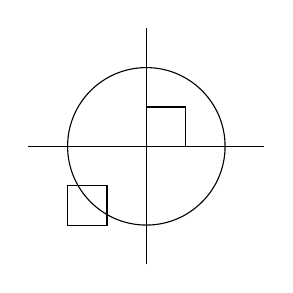
\begin{tikzpicture}
  \draw (-1.5,0) -- (1.5,0);
  \draw (0,-1.5) -- (0,1.5);
  \draw (0,0) circle [radius=1cm];
  \draw (0,0) rectangle (0.5,0.5);
  \draw (-0.5,-0.5) rectangle (-1,-1);
\end{tikzpicture}
\end{codeexample}

\bohs

% While this may be nice in other situations, this is not really leading
% anywhere with Karl's problem: First, we would need an awful lot of
% these rectangles and then there is the border that is not ``closed.''
也许在其他情况下这个方法还不错,但是并没有真的解决 Karl 的问题:首先我们需要很多很多矩形,并且边界处是不“闭合”的。

% So, Karl is about to resort to simply drawing four vertical and four
% horizontal lines using the nice |\draw| command, when he learns that
% there is a |grid| path construction operation.
所以,正当 Karl 准备用 \ltz{\\draw} 命令画四条横线、四条竖线时,他得知有一个 \ltz{grid} (网格)路径创建操作。

\eohs

% \subsection{Grid Path Construction}
\subsection{网格路径创建}

\bohs

% The |grid| path operation adds a grid to the current path. It will add
% lines making up a grid that fills the rectangle whose one corner is
% the current point and whose other corner is the point following the
% |grid| operation. For example, the code
% |\tikz \draw[step=2pt] (0,0) grid (10pt,10pt);| produces \tikz
% \draw[step=2pt] (0,0) grid (10pt,10pt);. Note how the optional
% argument for |\draw| can be used to specify a grid width (there are
% also |xstep| and |ystep| to define the steppings independently). As
% Karl will learn soon, there are \emph{lots} of things that can be
% influenced using such options.
|grid| 路径操作在当前路径加上网格。它会画出组成网格的线,|grid| 前后两个点坐标构成了网格矩形的两个对角。
比如,代码 \ltz{\\tikz \\draw[step=2pt] (0,0) grid (10pt,10pt);} 生成网格 \tikz \draw[step=2pt] (0,0) grid (10pt,10pt);。
注意到 \ltz{\\draw} 后面的选项,可以指定网格的宽度(还可以用 \ltz{xstep} 和 \ltz{ystep} 来分别设置网格间隔)。
正如 Karl 很快会学到的,用这些选项可以影响\emph{非常多}的事物。

% For Karl, the following code could be used:
Karl 可以用下面的代码:

\eohs

\begin{codeexample}[]
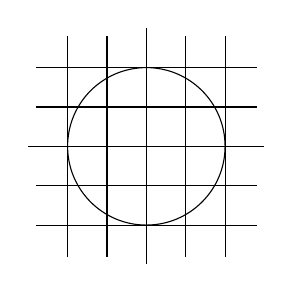
\begin{tikzpicture}
  \draw (-1.5,0) -- (1.5,0);
  \draw (0,-1.5) -- (0,1.5);
  \draw (0,0) circle [radius=1cm];
  \draw[step=.5cm] (-1.4,-1.4) grid (1.4,1.4);
\end{tikzpicture}
\end{codeexample}

\bohs

% Having another look at the desired picture, Karl notices that it would
% be nice for the grid to be more subdued. (His son told him that grids
% tend to be distracting if they are not subdued.) To subdue the grid,
% Karl adds two more options to the |\draw| command that draws the
% grid. First, he uses the color |gray| for the grid lines. Second, he
% reduces the line width to |very thin|. Finally, he swaps the ordering
% of the commands so that the grid is drawn first and everything else on
% top.
Karl 又看了一眼理想中的图片,他注意到,要是网格更柔和一点就好了。%
(他儿子告诉他,如果网格不柔和,会让人分心。)
为了让网格柔和,他又在 \ltz{\\draw} 后面加了两个选项。
首先他把网格线的颜色设为 \ltz{gray},然后将网格的线宽减到了 \ltz{very thin},最后,他调换了命令的顺序,先画网格,再在上面画其他的。

\eohs

\begin{codeexample}[]
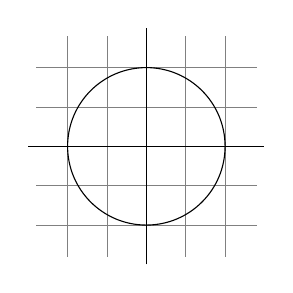
\begin{tikzpicture}
  \draw[step=.5cm,gray,very thin] (-1.4,-1.4) grid (1.4,1.4);
  \draw (-1.5,0) -- (1.5,0);
  \draw (0,-1.5) -- (0,1.5);
  \draw (0,0) circle [radius=1cm];
\end{tikzpicture}
\end{codeexample}


% \subsection{Adding a Touch of Style}
\subsection{添加一点样式}

\bohs

% Instead of the options |gray,very thin| Karl could also have
% said |help lines|. \emph{Styles} are predefined sets of options
% that can be used to organize how a graphic is drawn. By saying
% |help lines| you say ``use the style that I (or someone else)
% has set for drawing help lines.'' If Karl decides, at some later
% point, that grids should be drawn, say, using the color |blue!50|
% instead of |gray|, he could provide the following option somewhere:
除了用 \ltz{gray,very thin},Karl 还可以用 \ltz{help lines}。\emph{样式}就是预定义的选项集合,用来组织图形的绘制。
\ltz{help lines} 的意思是“使用我(或者其他人)已经设置好的绘制帮助线的样式”。
如果 Karl 之后打算用颜色 \ltz{blue!50} 而不是 \ltz{gray} 画网格,他可以用下面的选项:

\eohs

\begin{codeexample}[code only]
help lines/.style={color=blue!50,very thin}
\end{codeexample}

\bohs

% The effect of this ``style setter'' is that in the current
% scope or environment the |help lines| option has the same effect as
% |color=blue!50,very thin|.
这个“样式设置”的作用是,在当前作用域或环境下,\ltz{help lines} 的效果等同于 \ltz{color=blue!50,very thin}。

% Using styles makes your graphics code more flexible. You can
% change the way things look easily in a consistent manner.
% Normally, styles are defined at the beginning of a picture. However,
% you may sometimes wish to define a style globally, so that all
% pictures of your document can use this style. Then you can easily
% change the way all graphics look by changing this one style. In this
% situation you can use the |\tikzset| command at the beginning of the
% document as in
样式让图形代码更灵活,你可以用统一的方法更容易地修改图形的外观。
通常样式在图片开头定义,不过你有时候可能想定义一个全局样式,这样所有图片就可以用这个样式了,然后只改这个样式就能改所有图片的样式。
要想这样,你可以在文档开头用 \ltz{\tikzset} 命令:

\eohs

\begin{codeexample}[code only]
\tikzset{help lines/.style=very thin}
\end{codeexample}

\bohs

% To build a hierarchy of styles you can have one style use
% another. So in order to define a style |Karl's grid| that is based on
% the |grid| style Karl could say
你可以在一个样式中使用另一个样式,建立层级关系。
所以要在 \ltz{grid} 的基础上定义一个 \ltz{Karl's grid} 样式,可以这样写:

\eohs

\begin{codeexample}[code only]
\tikzset{Karl's grid/.style={help lines,color=blue!50}}
...
\draw[Karl's grid] (0,0) grid (5,5);
\end{codeexample}

\bohs

% Styles are made even more powerful by parametrization. This means
% that, like other options, styles can also be used with a
% parameter. For instance, Karl could parameterize his grid so that, by
% default, it is blue, but he could also use another color.
参数化可以让样式更强大,也就是说,像其他选项一样,样式也是能使用参数的。
比如,Karl 可以将他的网格样式参数化,默认蓝色,但也可以用另外一种颜色。

\eohs

\begin{codeexample}[code only]
\begin{tikzpicture}
  [Karl's grid/.style  ={help lines,color=#1!50},
   Karl's grid/.default=blue]

  \draw[Karl's grid]     (0,0) grid (1.5,2);
  \draw[Karl's grid=red] (2,0) grid (3.5,2);
\end{tikzpicture}
\end{codeexample}


% \subsection{Drawing Options}
\subsection{画图选项}

\bohs

% Karl wonders what other options there are that influence how a path is
% drawn. He saw already that the |color=|\meta{color} option can be used
% to set the line's color. The option |draw=|\meta{color} does nearly
% the same, only it sets the color for the lines only and a different
% color can be used for filling (Karl will need this when he fills the
% arc for the angle).
Karl 在想还有什么命令能够影响路径的绘制。
他已经注意到 \ltz{color=}{\color{blue} \meta{color}} 可以设置线的颜色,而 \ltz{draw=}{\color{blue} \meta{color}} 的作用几乎一样,只不过它只设置线的轮廓颜色,而填充颜色可以设置成另外一种(后面要填充弧线时,Karl 会用到这个)。

% He saw that the style |very thin| yields very thin lines. Karl is not
% really surprised by this and neither is he surprised to learn that |thin|
% yields thin lines,  |thick| yields thick lines, |very thick| yields
% very thick lines, |ultra thick| yields really, really thick lines and
% |ultra thin| yields lines that are so thin that low-resolution printers
% and displays will have trouble showing them. He wonders what gives
% lines of ``normal'' thickness. It turns out that |thin| is the correct
% choice, since it gives the same thickness as \TeX's |\hrule|
% command. Nevertheless, Karl would like to know whether there is 
% anything ``in the middle'' between |thin| and |thick|. There is:
% |semithick|.
Karl 还注意到 \ltz{very thin} 生成了很细的线,对此他并不奇怪,毕竟 \ltz{thin} 生成细线,\ltz{thick} 生成粗线,\ltz{very thick} 生成很粗的线,\ltz{ultra thick} 生成超粗的线,\ltz{ultra thin}生成超细的线,细到低分辨率的打印机和显示器都很难显示。
他想知道的是,线的“正常”粗细是多少。结果表明 \ltz{thin} 是正确的选项,因为它和 \TeX\ 的 \ltz{\\hrule} 命令生成的线粗细一样。
尽管如此,Karl 还是想知道,是否有选项在 \ltz{thin} 和 \ltz{thick} 中间。
事实上是有的,它就是 \ltz{semithick}。

% Another useful thing one can do with lines is to dash or dot them. For
% this, the two styles |dashed| and |dotted| can be used, yielding
% \tikz[baseline] \draw[dashed] (0,.5ex) -- ++(2em,0pt); and
% \tikz[baseline] \draw[dotted] (0,.5ex) 
% -- ++(2em,0pt);. Both options also exist in a loose and a dense
% version, called |loosely dashed|, |densely dashed|, |loosely dotted|,
% and |densely dotted|. If he really, really  needs to, Karl can also
% define much more complex dashing patterns with the |dash pattern|
% option, but his son insists that dashing is to be used with utmost
% care and mostly distracts. Karl's son claims that complicated dashing
% patterns are evil. Karl's students do not care about dashing patterns.
另一个有用的线样式是虚线和点线,可以用 \ltz{dashed} 生成 \tikz[baseline] \draw[dashed] (0,.5ex) -- ++(2em,0pt);,用 \ltz{dotted} 生成 \tikz[baseline] \draw[dotted] (0,.5ex) -- ++(2em,0pt);。
这两类线都有稀疏和紧密的版本,分别叫 \ltz{loosely dashed},\ltz{densely dashed},\ltz{loosely dotted} 和 \ltz{densely dotted}。
如果 Karl 真需要的话,他还可以用 \ltz{dash pattern} 设置更复杂的虚线图案。
不过他儿子说,虚线需要尽可能小心使用,并且最容易让人分心,复杂的虚线图案非常糟糕,毕竟 Karl 的学生并不关心虚线的图案。

\eohs

% \subsection{Arc Path Construction}
\subsection{弧线路径创建}

\bohs

% Our next obstacle is to draw the arc for the angle. For this, the
% |arc| path construction operation is useful, which draws part of a
% circle or ellipse. This |arc| operation is followed by options in
% brackets that specify the arc. An example would be \texttt{arc[start
%   angle=10, end angle=80, radius=10pt]}, which means exactly what it
% says. Karl obviously
% needs an arc from $0^\circ$ to $30^\circ$. The radius should be
% something relatively small, perhaps around one third of the circle's
% radius. When one uses the arc path construction operation, the
% specified arc will be added with its starting point at the current
% position. So, we first have to ``get there.''
我们的下一个问题是绘制角的弧线,这就要用到 \ltz{arc} 路径创建操作,可以画出圆或椭圆的一部分。
\ltz{arc} 后面方括号中的选项,指定了弧线的样子,一个例子是 \ltz{arc[start angle=10, end angle=80, radius=10pt]},其义如其名。
Karl 明显需要一个从 $0^\circ$ 到 $30^\circ$ 的弧线,半径要小一点,大概是圆的三分之一。
在使用弧线路径创建操作时,所画弧线的起始点是当前位置。因此,我们首先要“到达目标位置”。

\eohs

\begin{codeexample}[]
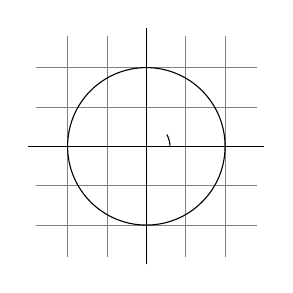
\begin{tikzpicture}
  \draw[step=.5cm,gray,very thin] (-1.4,-1.4) grid (1.4,1.4);
  \draw (-1.5,0) -- (1.5,0);
  \draw (0,-1.5) -- (0,1.5);
  \draw (0,0) circle [radius=1cm];
  \draw (3mm,0mm) arc [start angle=0, end angle=30, radius=3mm];
\end{tikzpicture}
\end{codeexample}

\bohs

% Karl thinks this is really a bit small and he cannot continue unless
% he learns how to do scaling. For this, he can add the |[scale=3]|
% option. He could add this option to each |\draw| command, but that
% would be awkward. Instead, he adds it to the whole environment, which
% causes this option to apply to everything within.
Karl 觉得图太小了,如果不学会如何放大,他就不能继续。
为此他可以加上 \ltz{[scale=3]} 的选项,可以把这个选项挨个加到所有 \ltz{\\draw} 命令上,但是这太蠢了。
所以他把它加到了整个环境上,这样就能将缩放效果应用到里面的所有元素了。

\eohs

\begin{codeexample}[]
\begin{tikzpicture}[scale=3]
  \draw[step=.5cm,gray,very thin] (-1.4,-1.4) grid (1.4,1.4);
  \draw (-1.5,0) -- (1.5,0);
  \draw (0,-1.5) -- (0,1.5);
  \draw (0,0) circle [radius=1cm];
  \draw (3mm,0mm) arc [start angle=0, end angle=30, radius=3mm];
\end{tikzpicture}
\end{codeexample}

\bohs

% As for circles, you can specify ``two'' radii in order to get an
% elliptical arc.
你可以给圆加上“两个”半径,就能得到椭圆弧线。

\eohs

\begin{codeexample}[]
  \tikz \draw (0,0) 
    arc [start angle=0, end angle=315, 
         x radius=1.75cm, y radius=1cm];
\end{codeexample}


% \subsection{Clipping a Path}
\subsection{剪裁路径}

\bohs

% In order to save space in this manual, it would be nice to clip Karl's
% graphics a bit so that we can focus on the ``interesting''
% parts. Clipping is pretty easy in \tikzname. You can use the |\clip|
% command to clip all subsequent drawing. It works like |\draw|, only it
% does not draw anything, but uses the given path to clip everything
% subsequently.
为了给本手册省点地方,最好能剪裁一下 Karl 的图片,这样我们就能只关注“感兴趣的”部分了。
在 \tikzname\ 中剪裁很容易,你可以用 \ltz{\\clip} 命令,剪裁之后画的所有图形。
它和 \ltz{\\draw} 很像,只不过它不画任何东西,而是按给定的路径,剪裁之后画的所有东西。

\eohs

\begin{codeexample}[]
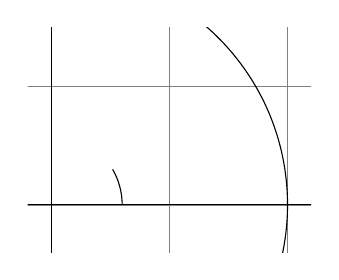
\begin{tikzpicture}[scale=3]
  \clip (-0.1,-0.2) rectangle (1.1,0.75);
  \draw[step=.5cm,gray,very thin] (-1.4,-1.4) grid (1.4,1.4);
  \draw (-1.5,0) -- (1.5,0);
  \draw (0,-1.5) -- (0,1.5);
  \draw (0,0) circle [radius=1cm];
  \draw (3mm,0mm) arc [start angle=0, end angle=30, radius=3mm];
\end{tikzpicture}
\end{codeexample}

\bohs

% You can also do both at the same time: Draw \emph{and} clip a
% path. For this, use the |\draw| command and add the |clip|
% option. (This is not the whole picture: You can also use the |\clip|
% command and add the |draw| option. Well, that is also not the whole
% picture: In reality, |\draw| is just a shorthand for |\path[draw]|
% and |\clip| is a shorthand for |\path[clip]| and you could also say
% |\path[draw,clip]|.) Here is an example:
你也可以同时绘制和剪裁路径,我们只需要给 \ltz{\\draw} 命令加上 \ltz{clip} 选项。%
(这并不是全部,你也可以用 \ltz{\\clip} 命令加上 \ltz{draw} 选项。不过这也还没完。
实际上, \ltz{\\draw} 只是 \ltz{\\path[draw]} 的简写, \ltz{\\clip} 是 \ltz{\\path[clip]} 的简写。因此你也可以用 \ltz{\\path[draw,clip]}。)
例子如下:

\eohs

\begin{codeexample}[]
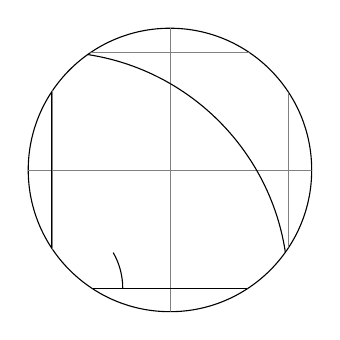
\begin{tikzpicture}[scale=3]
  \clip[draw] (0.5,0.5) circle (.6cm);
  \draw[step=.5cm,gray,very thin] (-1.4,-1.4) grid (1.4,1.4);
  \draw (-1.5,0) -- (1.5,0);
  \draw (0,-1.5) -- (0,1.5);
  \draw (0,0) circle [radius=1cm];
  \draw (3mm,0mm) arc [start angle=0, end angle=30, radius=3mm];
\end{tikzpicture}
\end{codeexample}


% \subsection{Parabola and Sine Path Construction}
\subsection{抛物线和正弦路径创建}

\bohs

% Although Karl does not need them for his picture, he is pleased to
% learn that there are |parabola| and |sin| and |cos| path operations for
% adding parabolas and sine and cosine curves to the current path. For the
% |parabola| operation, the current point will lie on the parabola as
% well as the point given after the parabola operation. Consider
% the following example:
尽管在这个图片里用不到,Karl 还是很高兴地了解到,路径操作还有 \ltz{parabola}、\ltz{sin} 和 \ltz{cos},也就是抛物线、正弦和余弦。
\ltz{parabola} 路径由前后两个点决定,见下例:

\eohs

\begin{codeexample}[]
\tikz \draw (0,0) rectangle (1,1)  (0,0) parabola (1,1);
\end{codeexample}

\bohs

% It is also possible to place the bend somewhere else:
也可以在某处加上弯曲(\ltz{bend}):

\eohs

\begin{codeexample}[]
\tikz \draw[x=1pt,y=1pt] (0,0) parabola bend (4,16) (6,12);
\end{codeexample}

\bohs

% The operations |sin| and |cos| add a sine or cosine curve in the interval
% $[0,\pi/2]$ such that the previous current point is at the start of
% the curve and the curve ends at the given end point. Here are two
% examples:
\ltz{sin} 或 \ltz{cos} 操作在两点间加上一条正弦或余弦曲线,区间为 $[0,\frac{\pi}{2}]$。
见如下两例:

\eohs

% A sine \tikz \draw[x=1ex,y=1ex] (0,0) sin (1.57,1); curve.
\begin{codeexample}[]
一条正弦 \tikz \draw[x=1ex,y=1ex] (0,0) sin (1.57,1); 曲线。
\end{codeexample}

\begin{codeexample}[]
\tikz \draw[x=1.57ex,y=1ex] (0,0) sin (1,1) cos (2,0) sin (3,-1) cos (4,0)
                            (0,1) cos (1,0) sin (2,-1) cos (3,0) sin (4,1);
\end{codeexample}


% \subsection{Filling and Drawing}
\subsection{填充和描边}

\bohs

% Returning to the picture, Karl now wants the angle to be ``filled''
% with a very light green. For this he uses |\fill| instead of
% |\draw|. Here is what Karl does:
回到之前的图片,Karl 现在想用浅绿色“填充”角。因此他使用 \ltz{\\fill} 而不是 \ltz{\\draw}。
如下:

\eohs

\begin{codeexample}[]
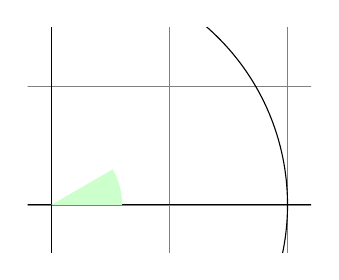
\begin{tikzpicture}[scale=3]
  \clip (-0.1,-0.2) rectangle (1.1,0.75);
  \draw[step=.5cm,gray,very thin] (-1.4,-1.4) grid (1.4,1.4);
  \draw (-1.5,0) -- (1.5,0);
  \draw (0,-1.5) -- (0,1.5);
  \draw (0,0) circle [radius=1cm];
  \fill[green!20!white] (0,0) -- (3mm,0mm)
    arc [start angle=0, end angle=30, radius=3mm] -- (0,0);
\end{tikzpicture}
\end{codeexample}

\bohs

% The color |green!20!white| means 20\% green and 80\% white mixed
% together. Such color expression are possible since \tikzname\ uses Uwe
% Kern's |xcolor| package, see the documentation of that package for
% details on color expressions.
颜色 \ltz{green!20!white} 意思是 20\% 的绿色混合 80\% 的白色。
\tikzname\ 中可以用这样的颜色表达式,因为已经导入了 Uwe Kern 的 \ltz{xcolor} 宏包,可以参考该宏包的文档,了解更多颜色表达式的细节。

% What would have happened, if Karl had not ``closed'' the path using
% |--(0,0)| at the end? In this case, the path is closed automatically,
% so this could have been omitted. Indeed, it would even have been
% better to write the following, instead:
如果 Karl 没有在结尾用 \ltz{--(0,0)} “闭合”路径,会怎么样?
此时路径会自动“闭合”,因此这句话可以略掉。
不过,如果像下面这样写,效果会更好:

\eohs

\begin{codeexample}[code only]
  \fill[green!20!white] (0,0) -- (3mm,0mm)
    arc [start angle=0, end angle=30, radius=3mm] -- cycle;
\end{codeexample}

\bohs

% The |--cycle| causes the current path to be closed (actually the
% current part of the current path) by smoothly joining the first and
% last point. To appreciate the difference, consider the following
% example:
\ltz{--cycle} 将当前路径闭合(实际上是当前路径的当前部分),也就是平滑地连接首尾两点。
可以通过下面的例子体会一下差别:

\eohs

\begin{codeexample}[]

\begin{tikzpicture}[line width=5pt]
  \draw (0,0) -- (1,0) -- (1,1) -- (0,0);
  \draw (2,0) -- (3,0) -- (3,1) -- cycle;
  \useasboundingbox (0,1.5); % make bounding box higher
\end{tikzpicture}
\end{codeexample}

\bohs

% You can also fill and draw a path at the same time using the
% |\filldraw| command. This will first draw the path, then fill it. This
% may not seem too useful, but you can specify different colors to be
% used for filling and for stroking. These are specified as optional
% arguments like this:
你也可以用 \ltz{\\filldraw} 命令同时对路径描边和填充。它会先描边,再填充。
这个看上去好像没什么用,不过这可以让你在描边和填充时用不同的颜色。
这些可以通过参数指定:

\eohs

\begin{codeexample}[]
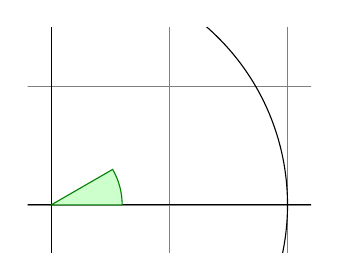
\begin{tikzpicture}[scale=3]
  \clip (-0.1,-0.2) rectangle (1.1,0.75);
  \draw[step=.5cm,gray,very thin] (-1.4,-1.4) grid (1.4,1.4);
  \draw (-1.5,0) -- (1.5,0);
  \draw (0,-1.5) -- (0,1.5);
  \draw (0,0) circle [radius=1cm];
  \filldraw[fill=green!20!white, draw=green!50!black] (0,0) -- (3mm,0mm)
    arc [start angle=0, end angle=30, radius=3mm] -- cycle;
\end{tikzpicture}
\end{codeexample}



% \subsection{Shading}
\subsection{渐变}

\bohs

% Karl briefly considers the possibility of making the angle ``more
% fancy'' by \emph{shading} it. Instead of filling the area with a uniform
% color, a smooth transition between different colors is used. For this,
% |\shade| and |\shadedraw|, for shading and drawing at the same time,
% can be used:
Karl 简单想了一下,有没有可能通过\emph{渐变}让这个角“更精致”。
填充时不是用单一的颜色,而是用平滑过渡的不同颜色。
\ltz{\\shade} 或 \ltz{\\shadedraw} 可以同时实现渐变和描边:

\eohs

\begin{codeexample}[]
  \tikz \shade (0,0) rectangle (2,1)  (3,0.5) circle (.5cm);
\end{codeexample}

\bohs

% The default shading is a smooth transition from gray to white. To
% specify different colors, you can use options:
默认的渐变是从灰色平滑过渡到白色,要指定不同的颜色,你可以加上选项:

\eohs

\begin{codeexample}[]

\begin{tikzpicture}[rounded corners,ultra thick]
  \shade[top color=yellow,bottom color=black] (0,0) rectangle +(2,1);
  \shade[left color=yellow,right color=black] (3,0) rectangle +(2,1);
  \shadedraw[inner color=yellow,outer color=black,draw=yellow] (6,0) rectangle +(2,1);
  \shade[ball color=green] (9,.5) circle (.5cm);
\end{tikzpicture}
\end{codeexample}

\bohs

% For Karl, the following might be appropriate:
对 Karl 来说,下面的设置也许更合适:

\eohs

\begin{codeexample}[]
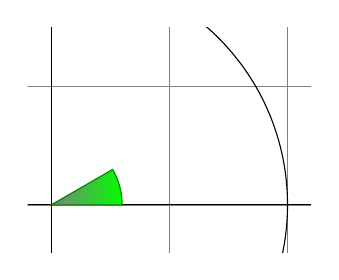
\begin{tikzpicture}[scale=3]
  \clip (-0.1,-0.2) rectangle (1.1,0.75);
  \draw[step=.5cm,gray,very thin] (-1.4,-1.4) grid (1.4,1.4);
  \draw (-1.5,0) -- (1.5,0);
  \draw (0,-1.5) -- (0,1.5);
  \draw (0,0) circle [radius=1cm];
  \shadedraw[left color=gray,right color=green, draw=green!50!black]
    (0,0) -- (3mm,0mm)
    arc [start angle=0, end angle=30, radius=3mm] -- cycle;
\end{tikzpicture}
\end{codeexample}

\bohs

% However, he wisely decides that shadings usually only distract without
% adding anything to the picture.
不过,他明智地认为,渐变通常只会使人分心,而不会对图片有任何加成。

\eohs

% \subsection{Specifying Coordinates}
\subsection{指定坐标}

\bohs

% Karl now wants to add the sine and cosine lines. He knows already that
% he can use the |color=| option to set the lines' colors. So, what is
% the best way to specify the coordinates?
Karl 现在想画上代表正弦值和余弦值的线段。
他已经知道可以用 \ltz{color=} 选项来设置线的轮廓颜色。
那么,用什么方法指定坐标最好呢?

% There are different ways of specifying coordinates. The easiest way is
% to say something like |(10pt,2cm)|. This means 10pt in $x$-direction
% and 2cm in $y$-directions. Alternatively, you can also leave out the
% units as in |(1,2)|, which means ``one times the current $x$-vector
% plus twice the current $y$-vector.'' These vectors default to 1cm in
% the $x$-direction and 1cm in the $y$-direction, respectively.
可以用不同的方法指定坐标。
最简单的就是 \ltz{(10pt,2cm)} 这种,意思是 $x$ 轴方向 10pt,$y$ 轴方向 2cm。
或者你也可以略掉单位,写成 \ltz{(1,2)},意思是“1 倍 $x$ 轴单位向量加上 2 倍 $y$ 轴单位向量”。
单位向量长度默认是 1 cm,$x$ 轴和 $y$ 轴都是如此。

% In order to specify points in polar coordinates, use the notation
% |(30:1cm)|, which means 1cm in direction 30 degree. This is obviously
% quite useful to ``get to the point $(\cos 30^\circ,\sin 30^\circ)$ on
% the circle.''
要用极坐标的方式指定点,可以用记号 \ltz{(30:1cm)},意思是沿 30 度角方向延伸 1 cm。
很明显,这个方法比“圆上一点 $(\cos 30^\circ, \sin 30^\circ)$”方便多了。

% You can add a single |+| sign in front of a coordinate or two of
% them as in |+(0cm,1cm)| or |++(2cm,0cm)|. Such coordinates are interpreted
% differently: The first form means ``1cm upwards from the previous
% specified position'' and the second means ``2cm to the right of the
% previous specified position, making this the new specified position.''
% For example, we can draw the sine line as follows:
你可以在坐标前加上一个或者两个 \ltz{+} 号,比如 \ltz{+(0cm,1cm)} 或者 \ltz{++(2cm,0cm)}。
这时坐标的含义就不一样了,前者表示“在之前指定位置的上方 1 cm”,后者表示“在之前指定位置的右侧 2 cm,并将该点作为新的指定位置”。
比如我们可以像下面这样,绘制代表正弦值的线段:

\eohs

\begin{codeexample}[]
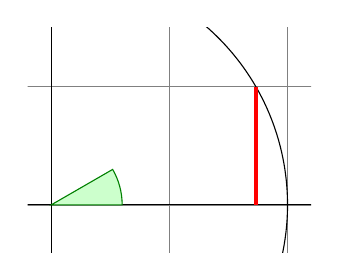
\begin{tikzpicture}[scale=3]
  \clip (-0.1,-0.2) rectangle (1.1,0.75);
  \draw[step=.5cm,gray,very thin] (-1.4,-1.4) grid (1.4,1.4);
  \draw (-1.5,0) -- (1.5,0);
  \draw (0,-1.5) -- (0,1.5);
  \draw (0,0) circle [radius=1cm];
  \filldraw[fill=green!20,draw=green!50!black] (0,0) -- (3mm,0mm)
      arc [start angle=0, end angle=30, radius=3mm] -- cycle;
  \draw[red,very thick] (30:1cm) -- +(0,-0.5);
\end{tikzpicture}
\end{codeexample}

\bohs

% Karl used the fact $\sin 30^\circ = 1/2$. However, he very much
% doubts that his students know this, so it would be nice to have a way
% of specifying ``the point straight down from |(30:1cm)| that lies on
% the $x$-axis.'' This is, indeed, possible using a special syntax: Karl
% can write \verb!(30:1cm |- 0,0)!. In general, the meaning of
% |(|\meta{p}\verb! |- !\meta{q}|)| is ``the intersection of a vertical
% line through $p$ and a horizontal line through $q$.''
Karl 这里用到了 $\sin 30^\circ = 1/2$,不过他觉得学生未必知道这个,所以他想,最好有方法能指定“\ltz{(30:1cm)} 到 $x$ 轴的垂足”。
这确实是可行的,需要用一个特殊的语法:\ltz{(30:1cm |- 0,0)}。
一般来说, {\color{blue} \texttt{(\meta{p} \ltz{\|-} \meta{q})}} 的意思是“过点 $p$ 的竖直线与过点 $q$ 的水平线的交点”。

% Next, let us draw the cosine line. One way would be to say
% \verb!(30:1cm |- 0,0) -- (0,0)!. Another way is the following: we
% ``continue'' from where the sine ends:
然后我们来画代表余弦值的线段。
一种方法是:\ltz{(30:1cm \|- 0,0) -- (0,0)}。
另一种方法如下:(我们接着正弦值线段那部分往下画)

\eohs

\begin{codeexample}[]
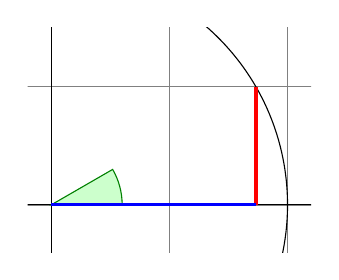
\begin{tikzpicture}[scale=3]
  \clip (-0.1,-0.2) rectangle (1.1,0.75);
  \draw[step=.5cm,gray,very thin] (-1.4,-1.4) grid (1.4,1.4);
  \draw (-1.5,0) -- (1.5,0);
  \draw (0,-1.5) -- (0,1.5);
  \draw (0,0) circle [radius=1cm];
  \filldraw[fill=green!20,draw=green!50!black] (0,0) -- (3mm,0mm)
      arc [start angle=0, end angle=30, radius=3mm] -- cycle;
  \draw[red,very thick]  (30:1cm) -- +(0,-0.5);
  \draw[blue,very thick] (30:1cm) ++(0,-0.5) -- (0,0);
\end{tikzpicture}
\end{codeexample}

\bohs

% Note that there is no |--| between |(30:1cm)| and |++(0,-0.5)|. In
% detail, this path is interpreted as follows: ``First, the |(30:1cm)|
% tells me to move by pen to $(\cos 30^\circ,1/2)$. Next, there comes
% another coordinate specification, so I move my pen there without drawing
% anything. This new point is half a unit down from the last position,
% thus it is at $(\cos 30^\circ,0)$. Finally, I move the pen to the
% origin, but this time drawing something (because of the |--|).''
注意,在 \ltz{(30:1cm)} 和 \ltz{++(0,-0.5)} 之间没有 \ltz{--}。
具体点说,这条路径应该这样解释:“首先,\ltz{(30:1cm)} 告诉我,要把笔移到 $(\cos 30^\circ,1/2)$;接着,我读到了另一个点坐标,因此将笔移动到新位置,并且什么也不画,新点在旧点下方的半个单位长度,也就是 $(\cos 30^\circ,0)$;最后,我把笔移到原点,不过这次要画出来(因为有 \ltz{--})。”

% To appreciate the difference between |+| and |++| consider the
% following example:
下例展示了 \ltz{+} 和 \ltz{++} 的区别:

\eohs

\begin{codeexample}[]

\begin{tikzpicture}
  \def\rectanglepath{-- ++(1cm,0cm)  -- ++(0cm,1cm)  -- ++(-1cm,0cm) -- cycle}
  \draw (0,0) \rectanglepath;
  \draw (1.5,0) \rectanglepath;
\end{tikzpicture}
\end{codeexample}

\bohs

% By comparison, when using a single |+|, the coordinates are different:
和 \ltz{++} 相比,使用 \ltz{+} 时,路径中的坐标有所不同:

\eohs

\begin{codeexample}[]

\begin{tikzpicture}
  \def\rectanglepath{-- +(1cm,0cm)  -- +(1cm,1cm)  -- +(0cm,1cm) -- cycle}
  \draw (0,0) \rectanglepath;
  \draw (1.5,0) \rectanglepath;
\end{tikzpicture}
\end{codeexample}

\bohs

% Naturally, all of this could have been written more clearly and more
% economically like this (either with a single of a double |+|):
当然,这些全都可以采用更加清晰精简的写法(既不用 \ltz{+} 也不用 \ltz{++}):

\eohs

\begin{codeexample}[]
\tikz \draw (0,0) rectangle +(1,1)  (1.5,0) rectangle +(1,1);
\end{codeexample}


% \subsection{Intersecting Paths}
\subsection{交叉路径}

\bohs

% Karl is left with the line for $\tan \alpha$, which seems difficult to
% specify using transformations and polar coordinates. The first -- and
% easiest -- thing he can do is so simply use the coordinate
% |(1,{tan(30)})| since \tikzname's math engine knows how to compute
% things like |tan(30)|. Note the added braces since, otherwise,
% \tikzname's parser would think that the first closing parenthesis ends
% the coordinate (in general, you need to add braces around components
% of coordinates when these components contain parentheses). 
现在 Karl 就剩 $\tan \alpha$ 对应的线段了,似乎用变换或者极坐标都不好画。
他能做的第一件事——也是最简单的一件事——就是用坐标 \ltz{(1,{tan(30)})},因为 \tikzname\ 的数学引擎知道如何计算 \ltz{tan(30)} 这样的式子。
注意外面加的花括号 \ltz{\{\}},这是因为 \tikzname\ 的语法分析器在读到第一个圆右括号 \ltz{)} 时,会当成是坐标的闭合(通常,如果坐标中的元素包含圆括号,你需要在它外面再套一层花括号)。

% Karl can, however, also use a more elaborate, but also more
% ``geometric'' way of computing the length of the orange line: He can
% specify intersections of paths as coordinates. The line for $\tan
% \alpha$ starts at $(1,0)$ 
% and goes upward to a point that is at the intersection of a line going
% ``up'' and a line going from the origin through |(30:1cm)|. Such
% computations are made available by the |intersections| library.
Karl 还可以用一种更“精致”也更“几何”的方法,来计算橙色线段的长度:
他可以指定路径的交点作为坐标。
$\tan \alpha$ 值对应的线段起点是 $(1,0)$,然后向“上”,直到和发自原点、指向 \ltz{(30:1cm)} 的线相交。
\ltz{intersections} 库可以支持这类运算。

% What Karl must do is to create two ``invisible'' paths that intersect
% at the position of interest. Creating paths that are not otherwise
% seen can be done using the |\path| command without any options like
% |draw| or |fill|. Then, Karl can add the |name path| option to the
% path for later reference. Once the paths have been constructed, Karl
% can use the |name intersections| to assign names to the coordinate for
% later reference.
Karl 要做的就是创建两条“隐形”路径,相交于目标位置。
创建隐形路径可以用 \ltz{\\path},不加任何 \ltz{draw} 或者 \ltz{fill} 这样的选项。
再给路径加上 \ltz{name path} 选项,用于后续的引用。
路径创建好后,Karl 就可以用 \ltz{name intersections} 选项来命名交点坐标,以供后续引用。

\eohs

\begin{codeexample}[code only]
\path [name path=upward line] (1,0) -- (1,1);
\path [name path=sloped line] (0,0) -- (30:1.5cm); % a bit longer, so that there is an intersection

\draw [name intersections={of=upward line and sloped line, by=x}]
  [very thick,orange] (1,0) -- (x);
\end{codeexample}


% \subsection{Adding Arrow Tips}
\subsection{添加箭头}

\bohs

% Karl now wants to add the little arrow tips at the end of the axes. He has
% noticed that in many plots, even in scientific journals, these arrow tips
% seem to be missing, presumably because the generating programs cannot
% produce them. Karl thinks arrow tips belong at the end of axes. His
% son agrees. His students do not care about arrow tips.
Karl 现在想给坐标轴末尾加个小箭头,他注意到在许多图中,甚至是科学期刊里的,都没有这些箭头,也许是生成的程序做不到这一点。
他觉得箭头应该在轴的尾端,他的儿子也同意,而他的学生并不关心箭头。

% It turns out that adding arrow tips is pretty easy: Karl adds the option
% |->| to the drawing commands for the axes:
实际上加箭头非常容易:
Karl 给画坐标轴的命令加上了一个 \ltz{->} 选项:

\eohs

\begin{codeexample}[]
\begin{tikzpicture}[scale=3]
  \clip (-0.1,-0.2) rectangle (1.1,1.51);
  \draw[step=.5cm,gray,very thin] (-1.4,-1.4) grid (1.4,1.4);
  \draw[->] (-1.5,0) -- (1.5,0);
  \draw[->] (0,-1.5) -- (0,1.5);
  \draw (0,0) circle [radius=1cm];
  \filldraw[fill=green!20,draw=green!50!black] (0,0) -- (3mm,0mm)
        arc [start angle=0, end angle=30, radius=3mm] -- cycle;
  \draw[red,very thick]    (30:1cm) -- +(0,-0.5);
  \draw[blue,very thick]   (30:1cm) ++(0,-0.5) -- (0,0);

  \path [name path=upward line] (1,0) -- (1,1);
  \path [name path=sloped line] (0,0) -- (30:1.5cm);
  \draw [name intersections={of=upward line and sloped line, by=x}]
        [very thick,orange] (1,0) -- (x);
\end{tikzpicture}
\end{codeexample}

\bohs

% If Karl had used the option |<-| instead of |->|, arrow tips would
% have been put at the beginning of the path. The option |<->| puts
% arrow tips at both ends of the path.
如果 Karl 用 \ltz{<-} 而非 \ltz{->},箭头就会加在路径开头,而 \ltz{<->} 则会把箭头加在路径两端。

% There are certain restrictions to the kind of paths to which arrow tips
% can be added. As a rule of thumb, you can add arrow tips only to a
% single open ``line.'' For example, you cannot add tips to,
% say, a rectangle or a circle. However, you can add arrow
% tips to curved paths and to paths that have several segments, as in
% the following examples:
对于可以添加箭头的路径类型,有一定的限制。
一般来说,你只能给一条开放的“线”添加箭头。比如,你不能给矩形或者圆加箭头。
不过你可以给曲线路径或者是多段路径加箭头,如下:

\eohs

\begin{codeexample}[]
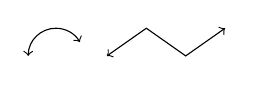
\begin{tikzpicture}
  \draw [<->] (0,0) arc [start angle=180, end angle=30, radius=10pt];
  \draw [<->] (1,0) -- (1.5cm,10pt) -- (2cm,0pt) -- (2.5cm,10pt);
\end{tikzpicture}
\end{codeexample}

\bohs

% Karl has a more detailed look at the arrow that \tikzname\ puts at the
% end. It looks like this when he zooms it: \tikz[baseline]
% \draw[->,line width=1pt] (0pt,.5ex) -- ++(10pt,0pt);. The shape seems
% vaguely familiar and, indeed, this is exactly the end of \TeX's
% standard arrow used in something like $f\colon A \to B$.
Karl 仔细地观察了一下 \tikzname\ 画在尾端的箭头。
放大后像这样:\tikz[baseline] \draw[->,line width=1pt] (0pt,.5ex) -- ++(10pt,0pt);。
形状似乎有点相似,而且事实上,这就是 \TeX\ 中标准箭头的尾端,用在 $f\colon A \to B$ 这样的地方。

% Karl likes the arrow, especially since it is not ``as thick'' as the
% arrows offered by many other packages. However, he expects that,
% sometimes, he might need to use some other kinds of arrow.
% To do so, Karl can say |>=|\meta{kind of end arrow tip}, where
% \meta{kind of end arrow tip} is a special arrow tip specification. For
% example, if Karl says |>=Stealth|, then he tells \tikzname\
% that he would like  ``stealth-fighter-like'' arrow tips:
Karl 喜欢这个箭头,尤其是它没有很多其他宏包中的“那么粗”。
不过他想,有时或许会用到其他类型的箭头。
为此,Karl 可以用~{\color{blue} \ltz{>=}\metazh{箭头尾端类型}},其中~{\color{blue} \metazh{箭头尾端类型}} 是一个特殊的箭头选项。
比方说,如果 Karl 用 \ltz{>=Stealth},那么这是在告诉 \tikzname\ 他喜欢“隐形战斗机式”的箭头:

\eohs

\begin{codeexample}[]
\begin{tikzpicture}[>=Stealth]
  \draw [->] (0,0) arc [start angle=180, end angle=30, radius=10pt];
  \draw [<<-,very thick] (1,0) -- (1.5cm,10pt) -- (2cm,0pt) -- (2.5cm,10pt);
\end{tikzpicture}
\end{codeexample}%>>

\bohs

% Karl wonders whether such a military name for the arrow type is really
% necessary. He is not really mollified when his son tells him that
% Microsoft's PowerPoint uses the same name. He decides to have his
% students discuss this at some point.
Karl 在想,箭头类型用这种军事上的名字是否真的有必要。
虽然 Karl 的儿子告诉他,微软的 PowerPoint 也用了相同的名字,可是他仍旧不能平静。
他决定有朝一日要让学生讨论一下这个话题。

% In addition to |Stealth| there are several other predefined kinds of
% arrow tips Karl can choose from, see Section~\ref{section-arrows}. Furthermore,
% he can define arrows types himself, if he needs new ones.
除了 \ltz{Stealth},Karl 还可以选择另外几种预先定义好的箭头,参见第 \ref{section-arrows} 小节。
此外,如果他需要新式箭头,也可以自己定义。

\eohs

% \subsection{Scoping}
\subsection{设置作用域}

\bohs

% Karl saw already that there are numerous graphic options that affect how
% paths are rendered. Often, he would like to apply certain options to
% a whole set of graphic commands. For example, Karl might wish to draw
% three paths using a |thick| pen, but would like everything else to
% be drawn ``normally.''
Karl 已经见到许多图形选项,用于改变路径的渲染方式。
他经常想在一套图形命令上用某些特定的图形选项。
比如说,他可能想拿一支粗(\ltz{thick})笔画三条路径,然后其他的都用“正常”选项。

% If Karl wishes to set a certain graphic option for the whole picture,
% he can simply pass this option to the |\tikz| command or to the
% |{tikzpicture}| environment (Gerda would pass the options to
% |\tikzpicture| and Hans passes them to |\starttikzpicture|). However,
% if Karl wants to apply graphic options to a local group, he put these
% commands inside a |{scope}| environment (Gerda uses |\scope| and
% |\endscope|, Hans uses |\startscope| and |\stopscope|). This
% environment takes graphic options as an optional argument and these
% options apply to everything inside the scope, but not to anything outside.
如果 Karl 想给整张图片设置一个特定的图形选项,那么他只需要把这个选项传给 \ltz{\\tikz} 或者放在 \ltz{\{tikzpicture\}} 环境中(Gerda 传给 \ltz{\\tikzpicture},Hans 则传给 \ltz{\\starttikzpicture})。
然而,如果 Karl 只想在局部的某组命令中使用这些选项,那么他就需要将这些命令放在 \ltz{\{scope\}} 环境中(Gerda 用 \ltz{\\scope},Hans 则用 \ltz{\\startscope} 和 \ltz{\\stopscope})。
这个环境把图形选项视为可选参数,只把他们应用在作用域内的命令中,对作用域外的没有影响。

% Here is an example:
例子如下:

\eohs

\begin{codeexample}[]
\begin{tikzpicture}[ultra thick]
  \draw (0,0) -- (0,1);
  \begin{scope}[thin]
    \draw (1,0) -- (1,1);
    \draw (2,0) -- (2,1);
  \end{scope}
  \draw (3,0) -- (3,1);
\end{tikzpicture}
\end{codeexample}

\bohs

% Scoping has another interesting effect: Any changes to the clipping
% area are local to the scope. Thus, if you say |\clip| somewhere inside
% a scope, the effect of the |\clip| command ends at the end of the
% scope. This is useful since there is no other way of ``enlarging'' the
% clipping area.
设置作用域还有另外一个有趣的影响:
对剪裁区域的任何改动,都局限在作用域内。
所以,如果你在作用域内的某个地方用了 \ltz{\\clip},那么剪裁的效果会在作用域外消失。
这很有用,因为只有这种方法能“放大”剪裁的区域。

% Karl has also already seen that giving options to commands like
% |\draw| apply only to that command. It turns out that the situation is
% slightly more complex. First, options to a command like |\draw| are
% not really options to the command, but they are ``path options'' and
% can be given anywhere on the path. So, instead of
% |\draw[thin] (0,0) -- (1,0);| one can also write
% |\draw (0,0) [thin] -- (1,0);| or |\draw (0,0) -- (1,0) [thin];|; all
% of these have the same effect. This might seem strange since in the
% last case, it would appear that the |thin| should take effect only
% ``after'' the line from $(0,0)$ to $(1,0)$ has been drawn. However,
% most graphic options only apply to the whole path. Indeed, if you say
% both |thin| and |thick| on the same path, the last option given will
% ``win.''
Karl 还发现,传给 \ltz{\\draw} 这类命令的选项,只对当前命令有用。
这下情况就有点复杂了。
首先,传给 \ltz{\\draw} 这类命令的选项,并不是真的作用于命令,而是“路径选项”,可以在路径的任何位置给出。
所以,除了用 \ltz{\\draw[thin] (0,0) -- (1,0);},你还可以写成 \ltz{\\draw (0,0) [thin] -- (1,0);} 或者 \ltz{\\draw (0,0) -- (1,0) [thin];}。
这些写法的效果是一样的。
看上去有点奇怪,按理说在最后一种写法中,\ltz{thin} 应该只对线段 \ltz{(0,0) -- (1,0)} 之后绘制的元素有影响。
事实上,如果你同时在路径中使用 \ltz{thin} 和 \ltz{thick},那么最后写的选项会“胜出”。

% When reading the above, Karl notices that only ``most'' graphic
% options apply to the whole path. Indeed, all transformation options do
% \emph{not} apply to the whole path, but only to ``everything following
% them on the path.'' We will have a more detailed look at this in a
% moment. Nevertheless, all options given during a path construction
% apply only to this path.

\eohs

\subsection{Transformations}

When you specify a  coordinate like |(1cm,1cm)|, where is that
coordinate placed on the page? To determine the position, \tikzname,
\TeX, and \textsc{pdf} or PostScript all apply certain transformations
to the given coordinate in order to determine the final position on
the page.

\tikzname\ provides numerous options that allow you to transform
coordinates in \tikzname's private coordinate system. For example, the
|xshift| option allows you to shift all subsequent points by a certain
amount:

\begin{codeexample}[]
\tikz \draw (0,0) -- (0,0.5) [xshift=2pt] (0,0) -- (0,0.5);
\end{codeexample}

It is important to note that you can change transformation ``in the
middle of a path,'' a feature that is not supported by \pdf\
or PostScript. The reason is that \tikzname\ keeps track of its own
transformation matrix.

Here is a more complicated example:
\begin{codeexample}[]

\begin{tikzpicture}[even odd rule,rounded corners=2pt,x=10pt,y=10pt]
  \filldraw[fill=yellow!80!black] (0,0)   rectangle (1,1)
        [xshift=5pt,yshift=5pt]   (0,0)   rectangle (1,1)
                    [rotate=30]   (-1,-1) rectangle (2,2);
\end{tikzpicture}
\end{codeexample}

The most useful transformations are |xshift| and |yshift| for
shifting, |shift| for shifting to a given point as in |shift={(1,0)}|
or |shift={+(0,0)}| (the braces are necessary so that \TeX\ does not
mistake the comma for separating options), |rotate| for rotating by a
certain angle (there is also a |rotate around| for rotating around a
given point), |scale| for scaling by a certain factor, |xscale| and
|yscale| for scaling only in the $x$- or $y$-direction (|xscale=-1| is
a flip), and |xslant| and |yslant| for slanting. If these
transformation and those that I have not mentioned are not
sufficient,  the |cm| option allows you to apply an arbitrary
transformation matrix. Karl's students, by the way, do not know what a
transformation matrix is.



\subsection{Repeating Things: For-Loops}

Karl's next aim is to add little ticks on the axes at positions $-1$,
$-1/2$, $1/2$, and $1$. For this, it would be nice to use some kind of
``loop,'' especially since he wishes to do the same thing at each of
these positions. There are different packages for doing this. \LaTeX\
has its own internal command for this, |pstricks| comes along with the
powerful |\multido| command. All of these can be used together with
\tikzname, so if you are familiar with them, feel free to
use them. \tikzname\ introduces yet another command, called |\foreach|,
which I introduced since I could never remember the syntax of the other
packages. |\foreach| is defined in the package |pgffor| and can be used
independently \tikzname, but \tikzname\ includes it automatically.

In its basic form, the |\foreach| command is easy to use:
\begin{codeexample}[]
\foreach \x in {1,2,3} {$x =\x$, }
\end{codeexample}

The general syntax is |\foreach| \meta{variable}| in {|\meta{list of
    values}|} |\meta{commands}. Inside the \meta{commands}, the
\meta{variable} will be assigned to the different values. If the
\meta{commands} do not start with a brace, everything up to the
next semicolon is used as \meta{commands}.

For Karl and the ticks on the axes, he could use the following code:

\begin{codeexample}[]
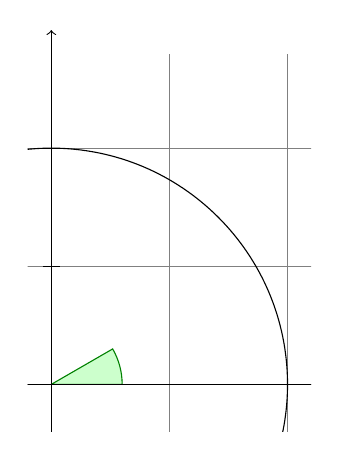
\begin{tikzpicture}[scale=3]
  \clip (-0.1,-0.2) rectangle (1.1,1.51);
  \draw[step=.5cm,gray,very thin] (-1.4,-1.4) grid (1.4,1.4);
  \filldraw[fill=green!20,draw=green!50!black] (0,0) -- (3mm,0mm)
      arc [start angle=0, end angle=30, radius=3mm] -- cycle;
  \draw[->] (-1.5,0) -- (1.5,0);
  \draw[->] (0,-1.5) -- (0,1.5);
  \draw (0,0) circle [radius=1cm];

  \foreach \x in {-1cm,-0.5cm,1cm}
    \draw (\x,-1pt) -- (\x,1pt);
  \foreach \y in {-1cm,-0.5cm,0.5cm,1cm}
    \draw (-1pt,\y) -- (1pt,\y);
\end{tikzpicture}
\end{codeexample}

As a matter of fact, there are many different ways of creating the
ticks. For example, Karl could have put the |\draw ...;| inside curly
braces. He could also have used, say,
\begin{codeexample}[code only]
\foreach \x in {-1,-0.5,1}
  \draw[xshift=\x cm] (0pt,-1pt) -- (0pt,1pt);
\end{codeexample}

Karl is curious what would happen in a more complicated situation
where there are, say, 20 ticks. It seems bothersome to explicitly
mention all these numbers in the set for |\foreach|. Indeed, it is
possible to use |...| inside the |\foreach| statement to iterate over
a large number of values (which must, however, be dimensionless
real numbers) as in the following example:

\begin{codeexample}[]
\tikz \foreach \x in {1,...,10}
        \draw (\x,0) circle (0.4cm);
\end{codeexample}

If you provide \emph{two} numbers before the |...|, the |\foreach|
statement will use their difference for the stepping:

\begin{codeexample}[]
\tikz \foreach \x in {-1,-0.5,...,1}
       \draw (\x cm,-1pt) -- (\x cm,1pt);
\end{codeexample}

We can also nest loops to create interesting effects:

\begin{codeexample}[]
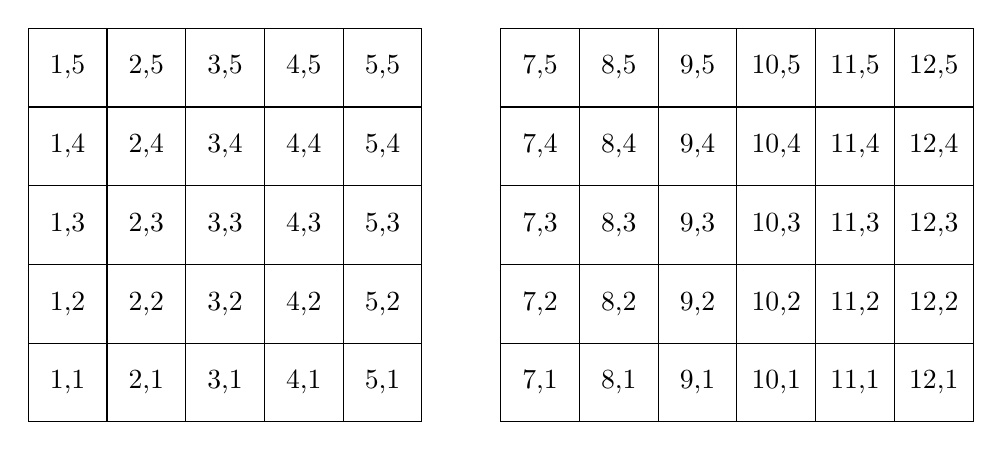
\begin{tikzpicture}
  \foreach \x in {1,2,...,5,7,8,...,12}
    \foreach \y in {1,...,5}
    {
      \draw (\x,\y) +(-.5,-.5) rectangle ++(.5,.5);
      \draw (\x,\y) node{\x,\y};
    }
\end{tikzpicture}
\end{codeexample}

The |\foreach| statement can do even trickier stuff, but the above
gives the idea.




\subsection{Adding Text}

Karl is, by now, quite satisfied with the picture. However, the most
important parts, namely the labels, are still missing!

\tikzname\ offers an easy-to-use and powerful system for adding text and,
more generally, complex shapes to a picture at specific positions. The
basic idea is the following: When \tikzname\ is constructing a path and
encounters the keyword |node| in the middle of a path, it
reads a \emph{node specification}. The keyword |node| is typically
followed by some options and then some text between curly braces. This
text is put inside a normal \TeX\ box (if the node specification
directly follows a coordinate, which is usually the case, \tikzname\ is
able to perform some magic so that it is even possible to use verbatim
text inside the boxes) and then placed at the current position, that
is, at the last specified position (possibly shifted a bit, according
to the given options). However, all nodes are drawn only after the
path has been completely drawn/filled/shaded/clipped/whatever.

\begin{codeexample}[]
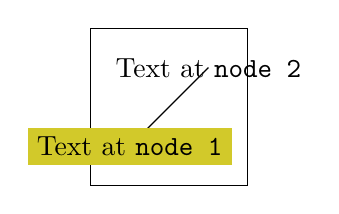
\begin{tikzpicture}
  \draw (0,0) rectangle (2,2);
  \draw (0.5,0.5) node [fill=yellow!80!black]
                       {Text at \verb!node 1!}
     -- (1.5,1.5) node {Text at \verb!node 2!};
\end{tikzpicture}
\end{codeexample}

Obviously, Karl would not only like to place nodes \emph{on} the last
specified position, but also to the left or the
right of these positions. For this, every node object that you
put in your picture is equipped with several \emph{anchors}. For
example, the |north| anchor is in the middle at the upper end of the shape,
the |south| anchor is at the bottom and the |north east| anchor is in
the upper right corner. When you give the option |anchor=north|, the
text will be placed such that this northern anchor will lie on the
current position and the text is, thus, below the current
position. Karl uses this to draw the ticks as follows:

\begin{codeexample}[]
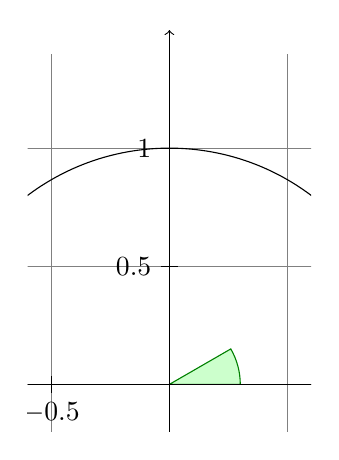
\begin{tikzpicture}[scale=3]
  \clip (-0.6,-0.2) rectangle (0.6,1.51);
  \draw[step=.5cm,help lines] (-1.4,-1.4) grid (1.4,1.4);
  \filldraw[fill=green!20,draw=green!50!black] (0,0) -- (3mm,0mm)
    arc [start angle=0, end angle=30, radius=3mm] -- cycle;
  \draw[->] (-1.5,0) -- (1.5,0);   \draw[->] (0,-1.5) -- (0,1.5);
  \draw (0,0) circle [radius=1cm];

  \foreach \x in {-1,-0.5,1}
    \draw (\x cm,1pt) -- (\x cm,-1pt) node[anchor=north] {$\x$};
  \foreach \y in {-1,-0.5,0.5,1}
    \draw (1pt,\y cm) -- (-1pt,\y cm) node[anchor=east] {$\y$};
\end{tikzpicture}
\end{codeexample}

This is quite nice, already. Using these anchors, Karl can now add
most of the other text elements. However, Karl thinks that, though
``correct,'' it is quite counter-intuitive that in order to place something
\emph{below} a given point, he has to use the \emph{north} anchor. For
this reason, there is an option called |below|, which does the
same as |anchor=north|. Similarly, |above right| does the same as
|anchor=south west|. In addition, |below| takes an optional
dimension argument. If given, the shape will additionally be shifted
downwards by the given amount. So, |below=1pt| can be used to put
a text label below some point and, additionally shift it  1pt
downwards.

Karl is not quite satisfied with the ticks. He would like to have
$1/2$ or $\frac{1}{2}$ shown instead of $0.5$, partly to show off the
nice capabilities of \TeX\ and \tikzname, partly because for positions
like $1/3$ or $\pi$ it is certainly very much preferable to have the
``mathematical'' tick there instead of just the ``numeric'' tick.
His students, on the other hand, prefer $0.5$ over $1/2$
since they are not too fond of fractions in general.

Karl now faces a problem: For the |\foreach| statement, the position
|\x| should still be given as |0.5| since \tikzname\ will not know where
|\frac{1}{2}| is supposed to be. On the other hand, the typeset text
should really be  |\frac{1}{2}|. To solve this problem, |\foreach|
offers a special syntax: Instead of having one variable |\x|, Karl can
specify two (or even more) variables separated by a slash as in
|\x / \xtext|. Then, the elements in the set over which |\foreach|
iterates must also be of the form \meta{first}|/|\meta{second}. In
each iteration, |\x| will be set to \meta{first} and |\xtext| will be
set to \meta{second}. If no \meta{second} is given, the \meta{first}
will be used again. So, here is the new code for the ticks:

\begin{codeexample}[]
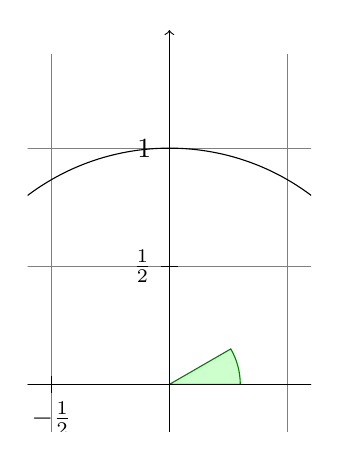
\begin{tikzpicture}[scale=3]
  \clip (-0.6,-0.2) rectangle (0.6,1.51);
  \draw[step=.5cm,help lines] (-1.4,-1.4) grid (1.4,1.4);
  \filldraw[fill=green!20,draw=green!50!black] (0,0) -- (3mm,0mm)
      arc [start angle=0, end angle=30, radius=3mm] -- cycle;
  \draw[->] (-1.5,0) -- (1.5,0); \draw[->] (0,-1.5) -- (0,1.5);
  \draw (0,0) circle [radius=1cm];

  \foreach \x/\xtext in {-1, -0.5/-\frac{1}{2}, 1}
    \draw (\x cm,1pt) -- (\x cm,-1pt) node[anchor=north] {$\xtext$};
  \foreach \y/\ytext in {-1, -0.5/-\frac{1}{2}, 0.5/\frac{1}{2}, 1}
    \draw (1pt,\y cm) -- (-1pt,\y cm) node[anchor=east] {$\ytext$};
\end{tikzpicture}
\end{codeexample}

Karl is quite pleased with the result, but his son points out that
this is still not perfectly satisfactory: The grid and the circle
interfere with the numbers and decrease their legibility. Karl is not
very concerned by this (his students do not even notice), but his son
insists that there is an easy solution: Karl can add the
|[fill=white]| option to fill out the background of the text shape
with a white color.

The next thing Karl wants to do is to add the labels like $\sin
\alpha$. For this, he would like to place a label ``in the middle of
the line.'' To do so, instead of specifying the label
|node {$\sin\alpha$}|  directly after one of the endpoints of the line
(which would place
the label at that endpoint), Karl can give the label directly after
the |--|, before the coordinate. By default, this places the label in
the middle of the line, but the |pos=| options can be used to modify
this. Also, options like |near start| and |near end| can be used to
modify this position:


\begin{codeexample}[]
\begin{tikzpicture}[scale=3]
  \clip (-2,-0.2) rectangle (2,0.8);
  \draw[step=.5cm,gray,very thin] (-1.4,-1.4) grid (1.4,1.4);
  \filldraw[fill=green!20,draw=green!50!black] (0,0) -- (3mm,0mm)
    arc [start angle=0, end angle=30, radius=3mm] -- cycle;
  \draw[->] (-1.5,0) -- (1.5,0) coordinate (x axis);
  \draw[->] (0,-1.5) -- (0,1.5) coordinate (y axis);
  \draw (0,0) circle [radius=1cm];

  \draw[very thick,red]
    (30:1cm) -- node[left=1pt,fill=white] {$\sin \alpha$} (30:1cm |- x axis);
  \draw[very thick,blue]
    (30:1cm |- x axis) -- node[below=2pt,fill=white] {$\cos \alpha$} (0,0);
  \path [name path=upward line] (1,0) -- (1,1);
  \path [name path=sloped line] (0,0) -- (30:1.5cm);
  \draw [name intersections={of=upward line and sloped line, by=t}]
    [very thick,orange] (1,0) -- node [right=1pt,fill=white]
    {$\displaystyle \tan \alpha \color{black}=
      \frac{{\color{red}\sin \alpha}}{\color{blue}\cos \alpha}$} (t);

  \draw (0,0) -- (t);

  \foreach \x/\xtext in {-1, -0.5/-\frac{1}{2}, 1}
    \draw (\x cm,1pt) -- (\x cm,-1pt) node[anchor=north,fill=white] {$\xtext$};
  \foreach \y/\ytext in {-1, -0.5/-\frac{1}{2}, 0.5/\frac{1}{2}, 1}
    \draw (1pt,\y cm) -- (-1pt,\y cm) node[anchor=east,fill=white] {$\ytext$};
\end{tikzpicture}
\end{codeexample}

You can also position labels on curves and, by adding the |sloped|
option, have them rotated such that they match the line's slope. Here
is an example:

\begin{codeexample}[]
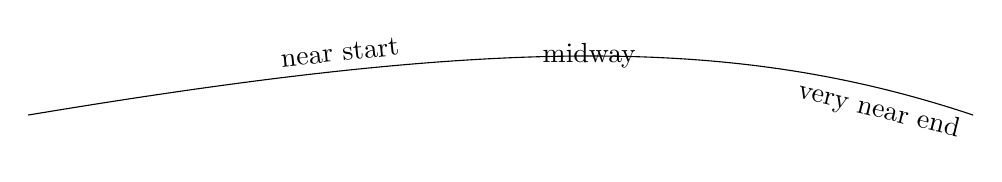
\begin{tikzpicture}
  \draw (0,0) .. controls (6,1) and (9,1) ..
    node[near start,sloped,above] {near start}
    node {midway}
    node[very near end,sloped,below] {very near end} (12,0);
\end{tikzpicture}
\end{codeexample}

It remains to draw the explanatory text at the right of the
picture. The main difficulty here lies in limiting the width of the
text ``label,'' which is quite long, so that line breaking is
used. Fortunately, Karl can use the option |text width=6cm| to get the
desired effect. So, here is the full code:

\begin{codeexample}[code only]
\begin{tikzpicture}
  [scale=3,line cap=round,
  % Styles
  axes/.style=,
  important line/.style={very thick},
  information text/.style={rounded corners,fill=red!10,inner sep=1ex}]

  % Colors
  \colorlet{anglecolor}{green!50!black}
  \colorlet{sincolor}{red}
  \colorlet{tancolor}{orange!80!black}
  \colorlet{coscolor}{blue}

  % The graphic
  \draw[help lines,step=0.5cm] (-1.4,-1.4) grid (1.4,1.4);

  \draw (0,0) circle [radius=1cm];

  \begin{scope}[axes]
    \draw[->] (-1.5,0) -- (1.5,0) node[right] {$x$} coordinate(x axis);
    \draw[->] (0,-1.5) -- (0,1.5) node[above] {$y$} coordinate(y axis);

    \foreach \x/\xtext in {-1, -.5/-\frac{1}{2}, 1}
      \draw[xshift=\x cm] (0pt,1pt) -- (0pt,-1pt) node[below,fill=white] {$\xtext$};

    \foreach \y/\ytext in {-1, -.5/-\frac{1}{2}, .5/\frac{1}{2}, 1}
      \draw[yshift=\y cm] (1pt,0pt) -- (-1pt,0pt) node[left,fill=white] {$\ytext$};
  \end{scope}

  \filldraw[fill=green!20,draw=anglecolor] (0,0) -- (3mm,0pt)
    arc [start angle=0, end angle=30, radius=3mm];
  \draw (15:2mm) node[anglecolor] {$\alpha$};

  \draw[important line,sincolor]
    (30:1cm) -- node[left=1pt,fill=white] {$\sin \alpha$} (30:1cm |- x axis);

  \draw[important line,coscolor]
    (30:1cm |- x axis) -- node[below=2pt,fill=white] {$\cos \alpha$} (0,0);

  \path [name path=upward line] (1,0) -- (1,1);
  \path [name path=sloped line] (0,0) -- (30:1.5cm);
  \draw [name intersections={of=upward line and sloped line, by=t}]
    [very thick,orange] (1,0) -- node [right=1pt,fill=white]
    {$\displaystyle \tan \alpha \color{black}=
      \frac{{\color{red}\sin \alpha}}{\color{blue}\cos \alpha}$} (t);

  \draw (0,0) -- (t);

  \draw[xshift=1.85cm]
    node[right,text width=6cm,information text]
    {
      The {\color{anglecolor} angle $\alpha$} is $30^\circ$ in the
      example ($\pi/6$ in radians). The {\color{sincolor}sine of
        $\alpha$}, which is the height of the red line, is
      \[
      {\color{sincolor} \sin \alpha} = 1/2.
      \]
      By the Theorem of Pythagoras ...
    };
\end{tikzpicture}
\end{codeexample}



\subsection{Pics: The Angle Revisited}

Karl expects that the code of certain parts of the picture he created
might be so useful that he might wish to reuse them in the
future. A natural thing to do is to create \TeX\ macros that store
the code he wishes to reuse. However, \tikzname\ offers another way
that is integrated directly into its parser: pics!

A ``pic'' is ``not quite a full picture,'' hence the short name. The
idea is that a pic is simply some code that you can add to a picture
at different places using the |pic| command whose syntax is almost
identical to the |node| command. The main difference is that instead
of specifying some text in curly braces that should be shown, you
specify the name of a predefined picture that should be shown. 

Defining new pics is easy enough, see Section~\ref{section-pics}, but
right now we just want to use one such predefined pic: the |angle|
pic. As the name suggests, it is a small drawing of an angle
consisting of a little wedge and an arc together with some text (Karl
needs to load the |angle| library and the |quotes| for the following
examples). What makes this pic useful is the fact that the size of the
wedge will be computed automatically.

The |angle| pic draws an angle between the two lines $BA$ and $BC$,
where $A$, $B$, and $C$ are three coordinates. In our case, $B$ is the
origin, $A$ is somewhere on the $x$-axis and $C$ is somewhere on a
line at $30^\circ$. 

\begin{codeexample}[]
\begin{tikzpicture}[scale=3]
  \coordinate (A) at (1,0);
  \coordinate (B) at (0,0);
  \coordinate (C) at (30:1cm);

  \draw (A) -- (B) -- (C)
        pic [draw=green!50!black, fill=green!20, angle radius=9mm,
             "$\alpha$"] {angle = A--B--C};
\end{tikzpicture}  
\end{codeexample}

Let us see, what is happening here. First we have specified three
\emph{coordinates} using the |\coordinate| command. It allows us to
name a specific coordinate in the picture. Then comes something that
starts as a normal |\draw|, but then comes the |pic| command. This
command gets lots of options and, in curly braces, comes the most
important point: We specify that we want to add an |angle| pic and
this angle should be between the points we named |A|, |B|, and |C| (we
could use other names). Note that the text that we want to be shown in
the pic is specified in quotes inside the options of the |pic|, not
inside the curly braces.

To learn more about pics, please see Section~\ref{section-pics}.